\chapter{Design of the Algorithm}
\label{chap:design}

\section{Analysis of an image}

\subsection{Using Harris corner detector}
The analysis of an image begins with applying the Harris detector on it. It will compute a given score for each pixel of the image, the higher the score, the greater the chance that pixel represents a corner.\\
Using these values we will have to determine a subset of pixels that will represent the Harris mask of the image.
Experimentally, we have established that all the points which have a value greater than $0.01 * max\_image\_value$ are to be part of the subset.\\
As an example, Figure~\ref{fig:beforeHarris} shows a normal image of a woman's face, while Figure~\ref{fig:afterHarris} shows the corresponding pixels that form the corner mask. \\

\begin{figure}[ht!]
\centering
\begin{minipage}{.5\textwidth}
	\centering
	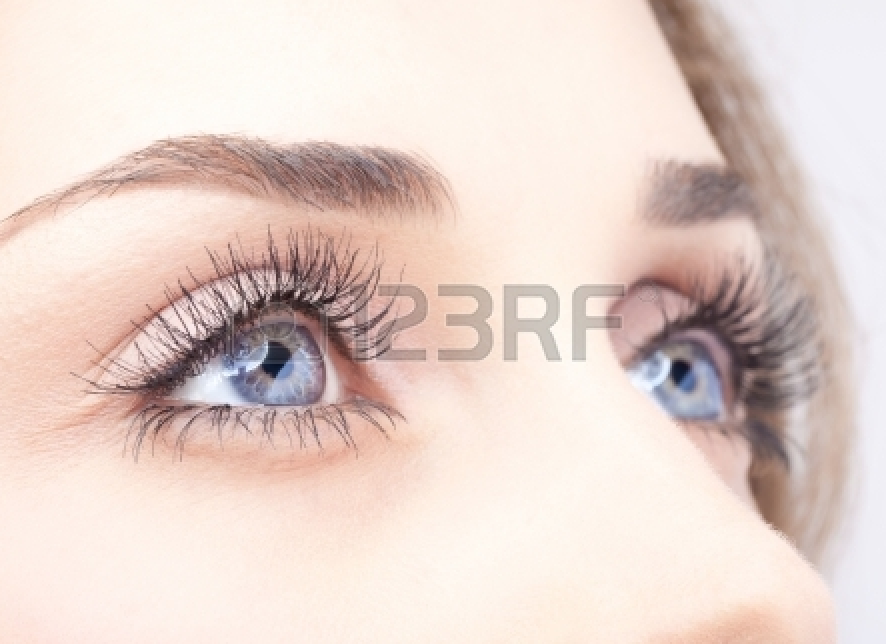
\includegraphics[width=.8\linewidth]{images/beforeHarris.png}
	\caption{Sample image}
	\label{fig:beforeHarris}
\end{minipage}%
\begin{minipage}{.5\textwidth}
	\centering
	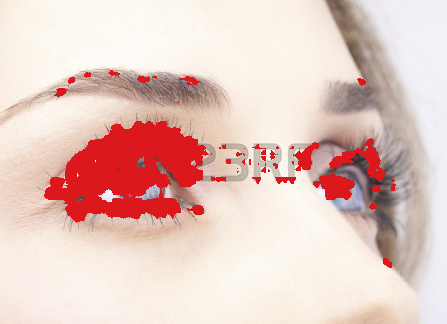
\includegraphics[width=.8\linewidth]{images/afterHarris.png}
	\caption{Harris corner mask applied }
	\label{fig:afterHarris}
\end{minipage}
\end{figure}

As it can be seen from the image, the corner mask centers around the interest points in the image, the eyes and the eyelashes, while leaving the smooth surfaces (the skin) unmarked.

Another observation is that possible watermarks can be present in the image (as seen above), which, of course, the mask detects (they are center pieces of the image, and the corner algorithm cannot determine that they have no real connection with the image).

Furthermore, in some cases the watermark might contain all (or at least a vast majority of) the points in the mask (as seen in Figure~\ref{fig:watermarkHarris}). To avoid such a behavior, I have split the image into 9 sub images (three rows and three columns of identical dimensions) and the Harris mask is applied to each of these.

\begin{figure}[ht!]
\centering
\begin{minipage}{.5\textwidth}
	\centering
	
\includegraphics[width=.8\linewidth]{images/watermarkHarris.png}
	\caption{Single image}
	\label{fig:watermarkHarris}
\end{minipage}%
\begin{minipage}{.5\textwidth}
	\centering
	
\includegraphics[width=.8\linewidth]{images/watermarkHarris9.png}
	\caption{9 subimages}
	\label{fig:watermarkHarris9}
\end{minipage}
\end{figure}

This determines the corner mask to also contain pixels from the center of the image (some of which, unfortunately, are also a watermark).
This partitioning scheme can be further extended by having a weighted selection of corner points: a larger number from the center of the image (where the interest point is) and a
smaller one from the corners.


\subsection{Using SIFT keypoints and descriptors}

As we have seen, the SIFT algorithm computes the keypoints of an image, and then the descriptors of these keypoints. Due to the high similarity nature of our problem, we do not want to compute the keypoints for the entire image, but filter them based on the corner mask determined in the previous section (as observed in Figure~\ref{fig:messiSift} and Figure~\ref{fig:messiCornerSift})

\begin{figure}[ht!]
\centering
\begin{minipage}{.5\textwidth}
	\centering
	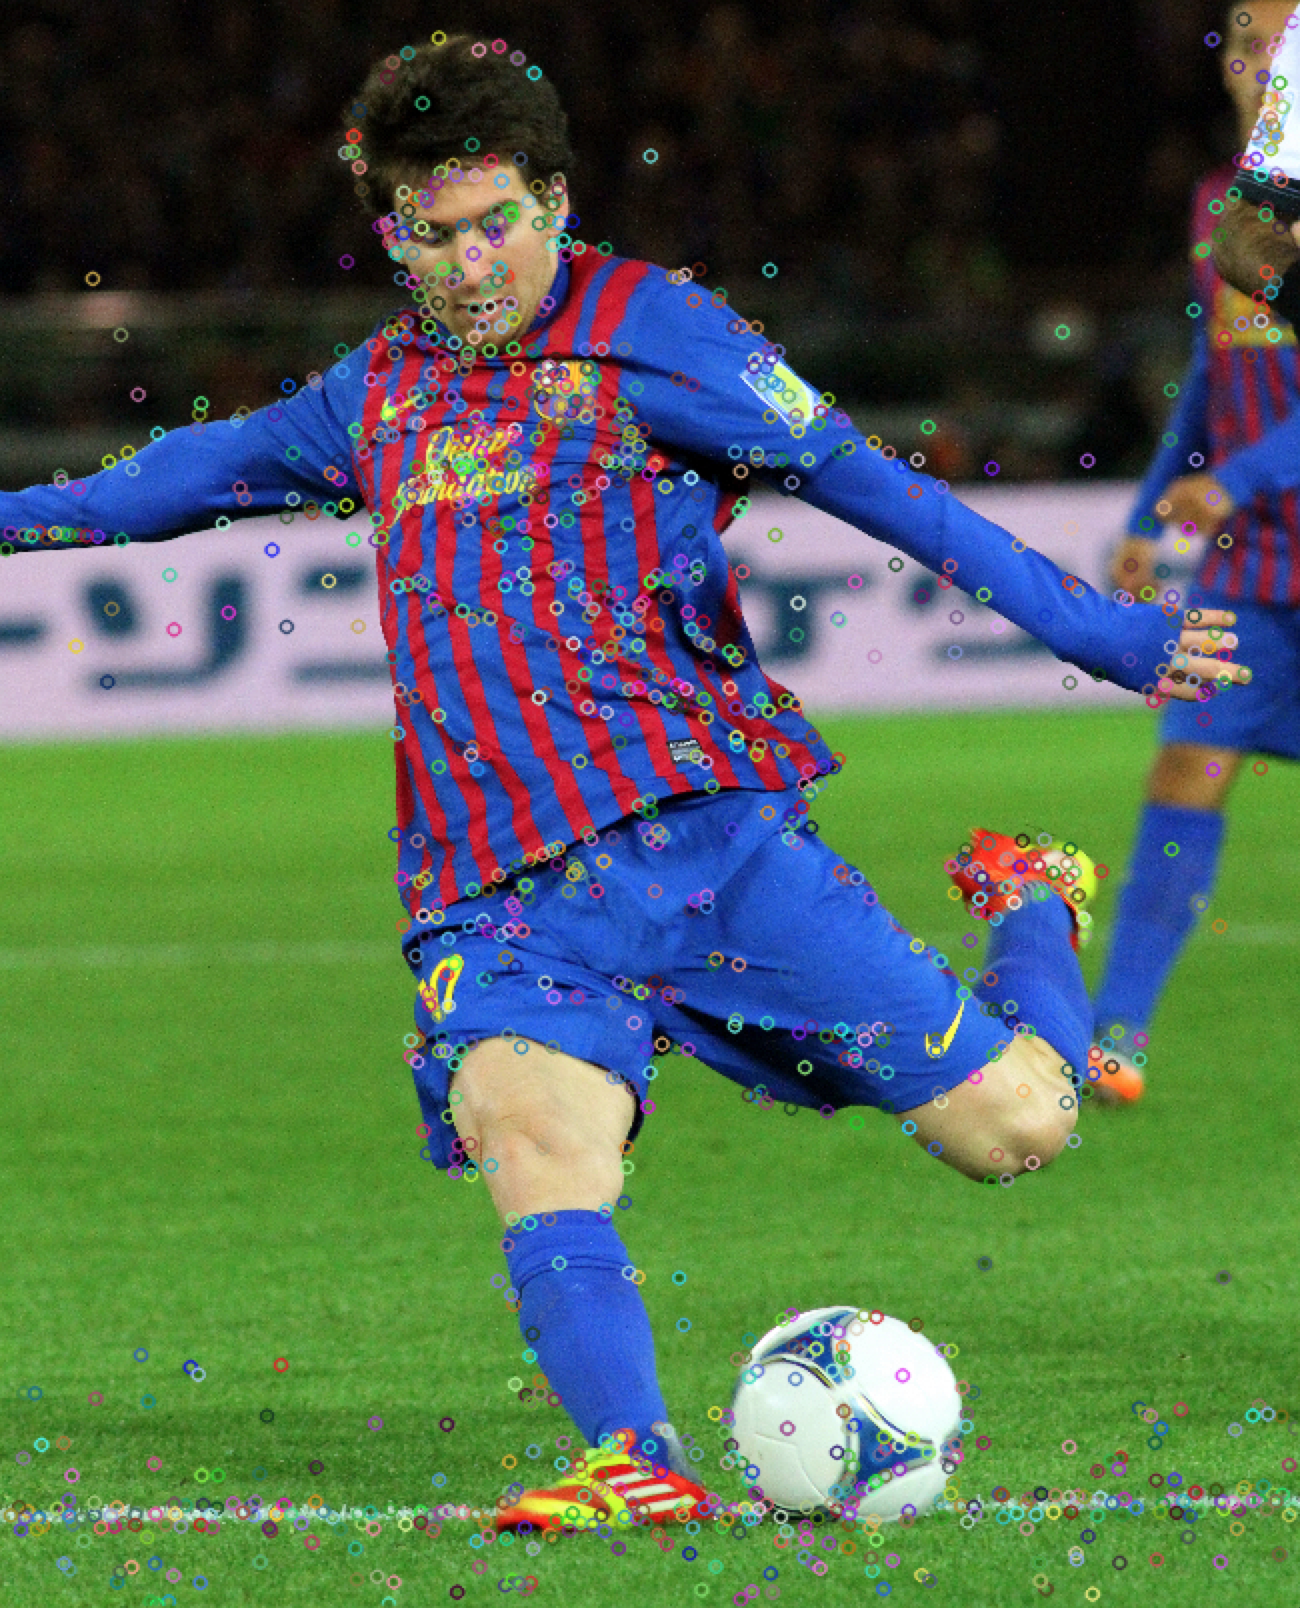
\includegraphics[width=.8\linewidth]{images/messiSift.png}
	\caption{SIFT keypoints for the\\ entire image}
	\label{fig:messiSift}
\end{minipage}%
\begin{minipage}{.5\textwidth}
	\centering
	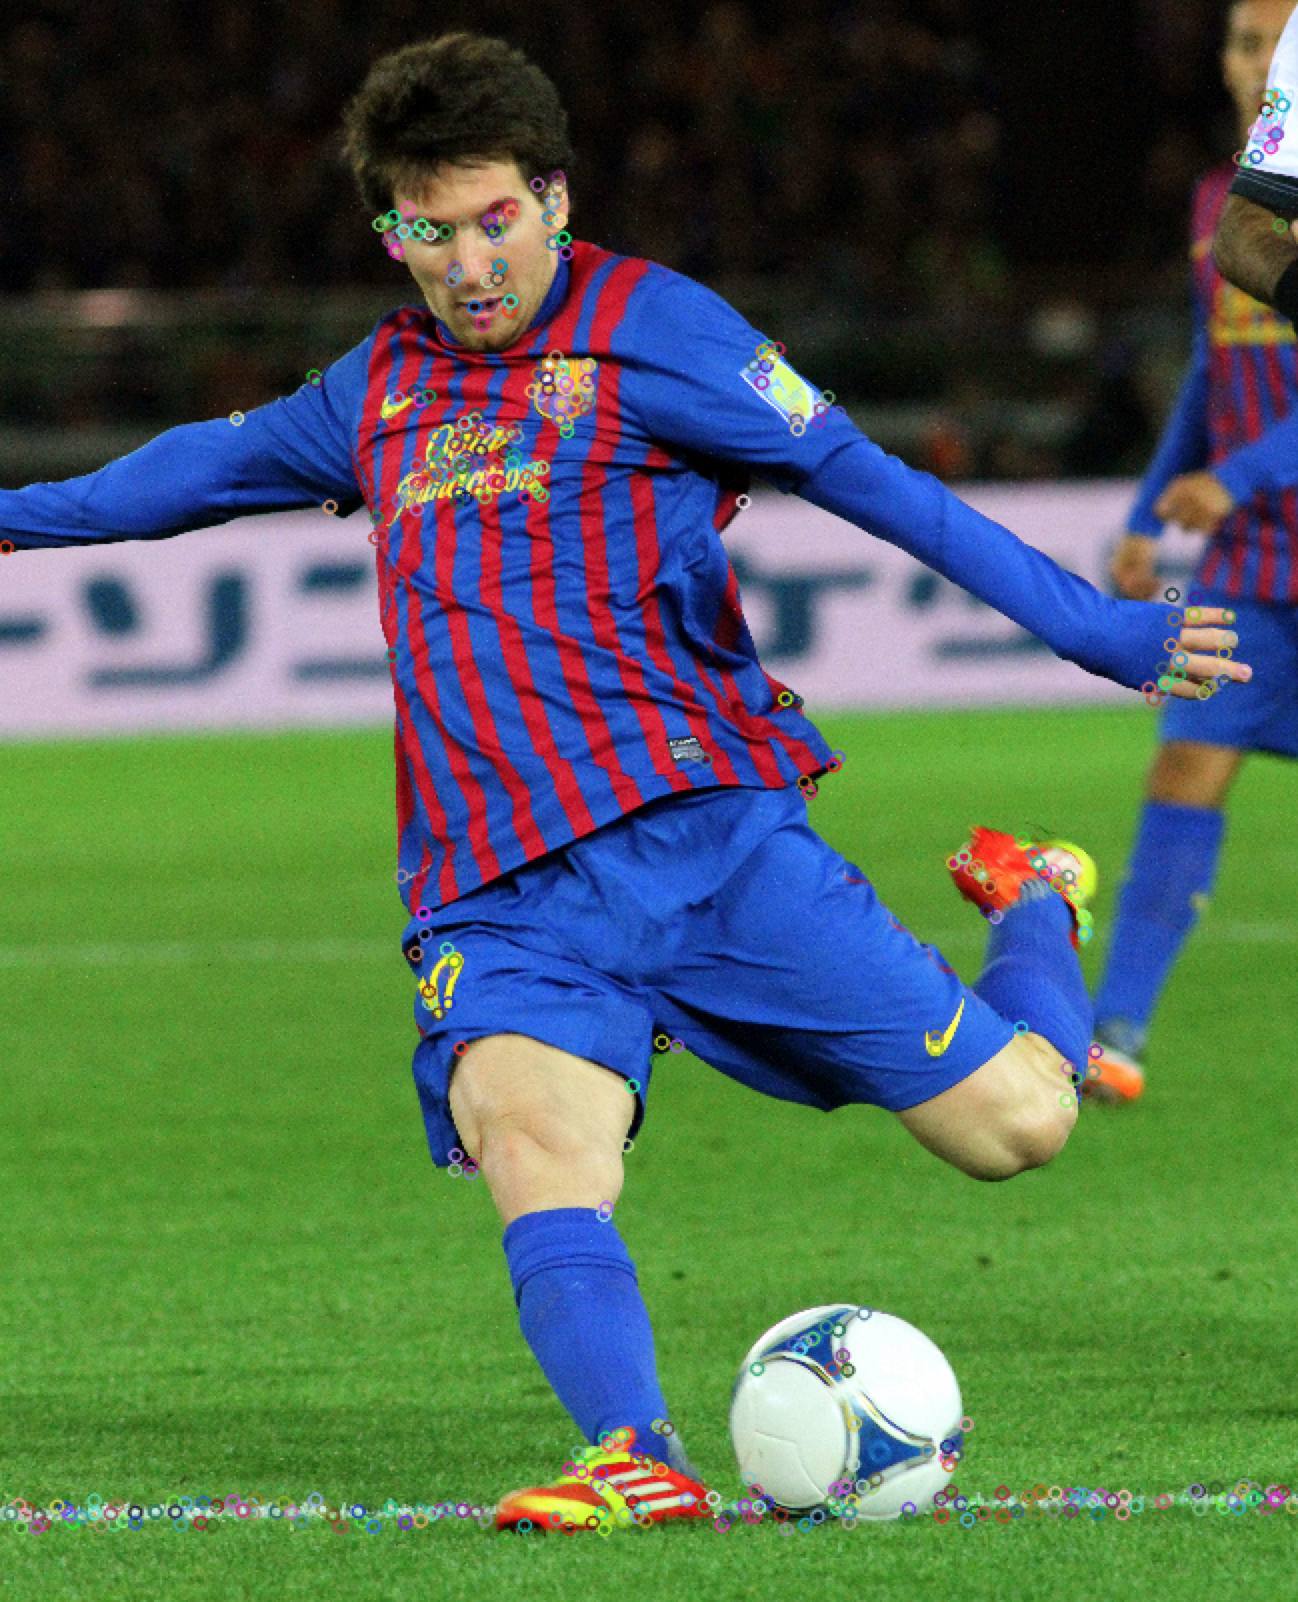
\includegraphics[width=.8\linewidth]{images/messiCornerSift.png}
	\caption{SIFT keypoints with\\ corner mask}
	\label{fig:messiCornerSift}
\end{minipage}
\end{figure}

The SIFT descriptors are then computed for each keypoint located in the corner mask and this will be the information stored for a certain image.

\subsection{Using SURF keypoints and descriptors}

As stated in \nameref{chap:relatedWork}, SURF descriptors have a similar performance as the SIFT ones, but are faster and have a lower dimensionality, so we might want to do a comparison between the two.
In Figure~\ref{fig:messiSurf} and Figure~\ref{fig:messiCornerSurf} we can see an example of the SURF keypoints applied on the above image, and the corner-filtered SURF keypoints.

\begin{figure}[ht!]
\centering
\begin{minipage}{.5\textwidth}
	\centering
	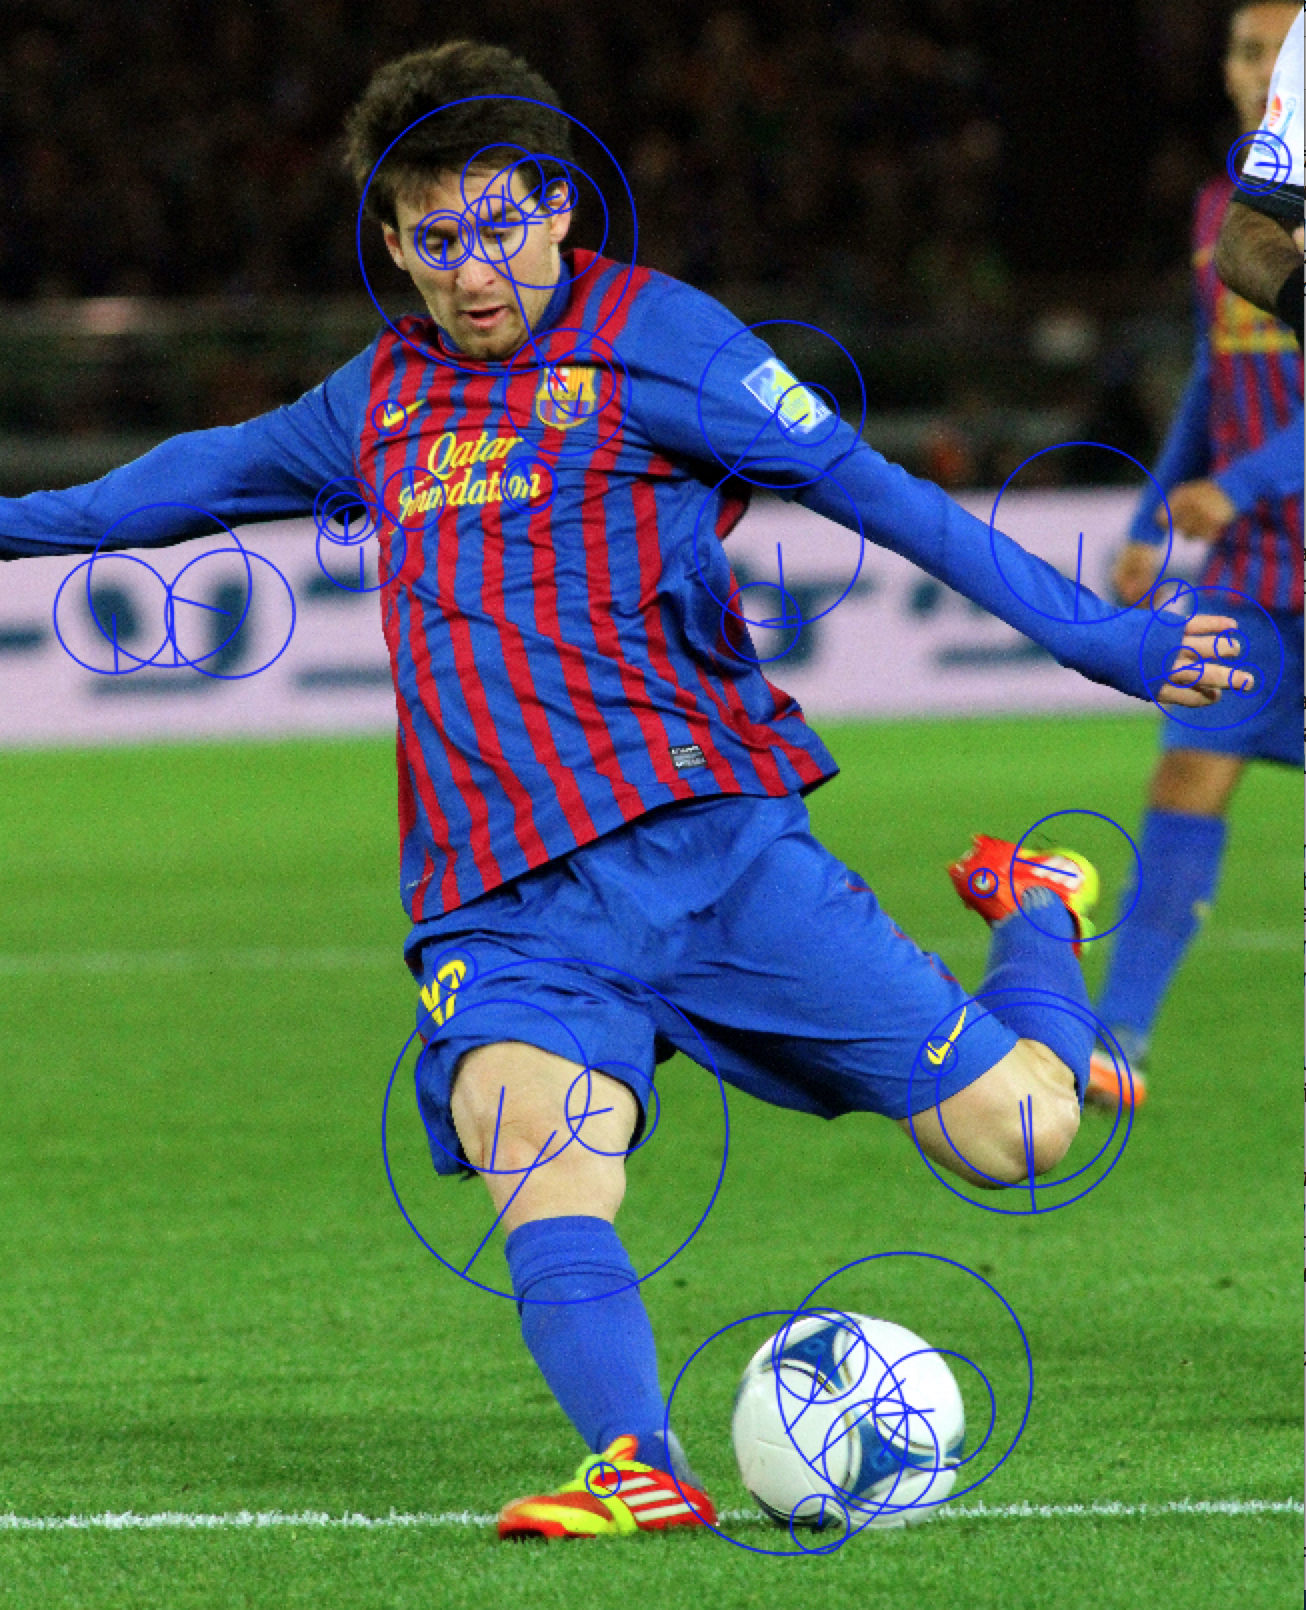
\includegraphics[width=.8\linewidth]{images/messiSurf.png}
	\caption{SURF keypoints for the\\ entire image}
	\label{fig:messiSurf}
\end{minipage}%
\begin{minipage}{.5\textwidth}
	\centering
	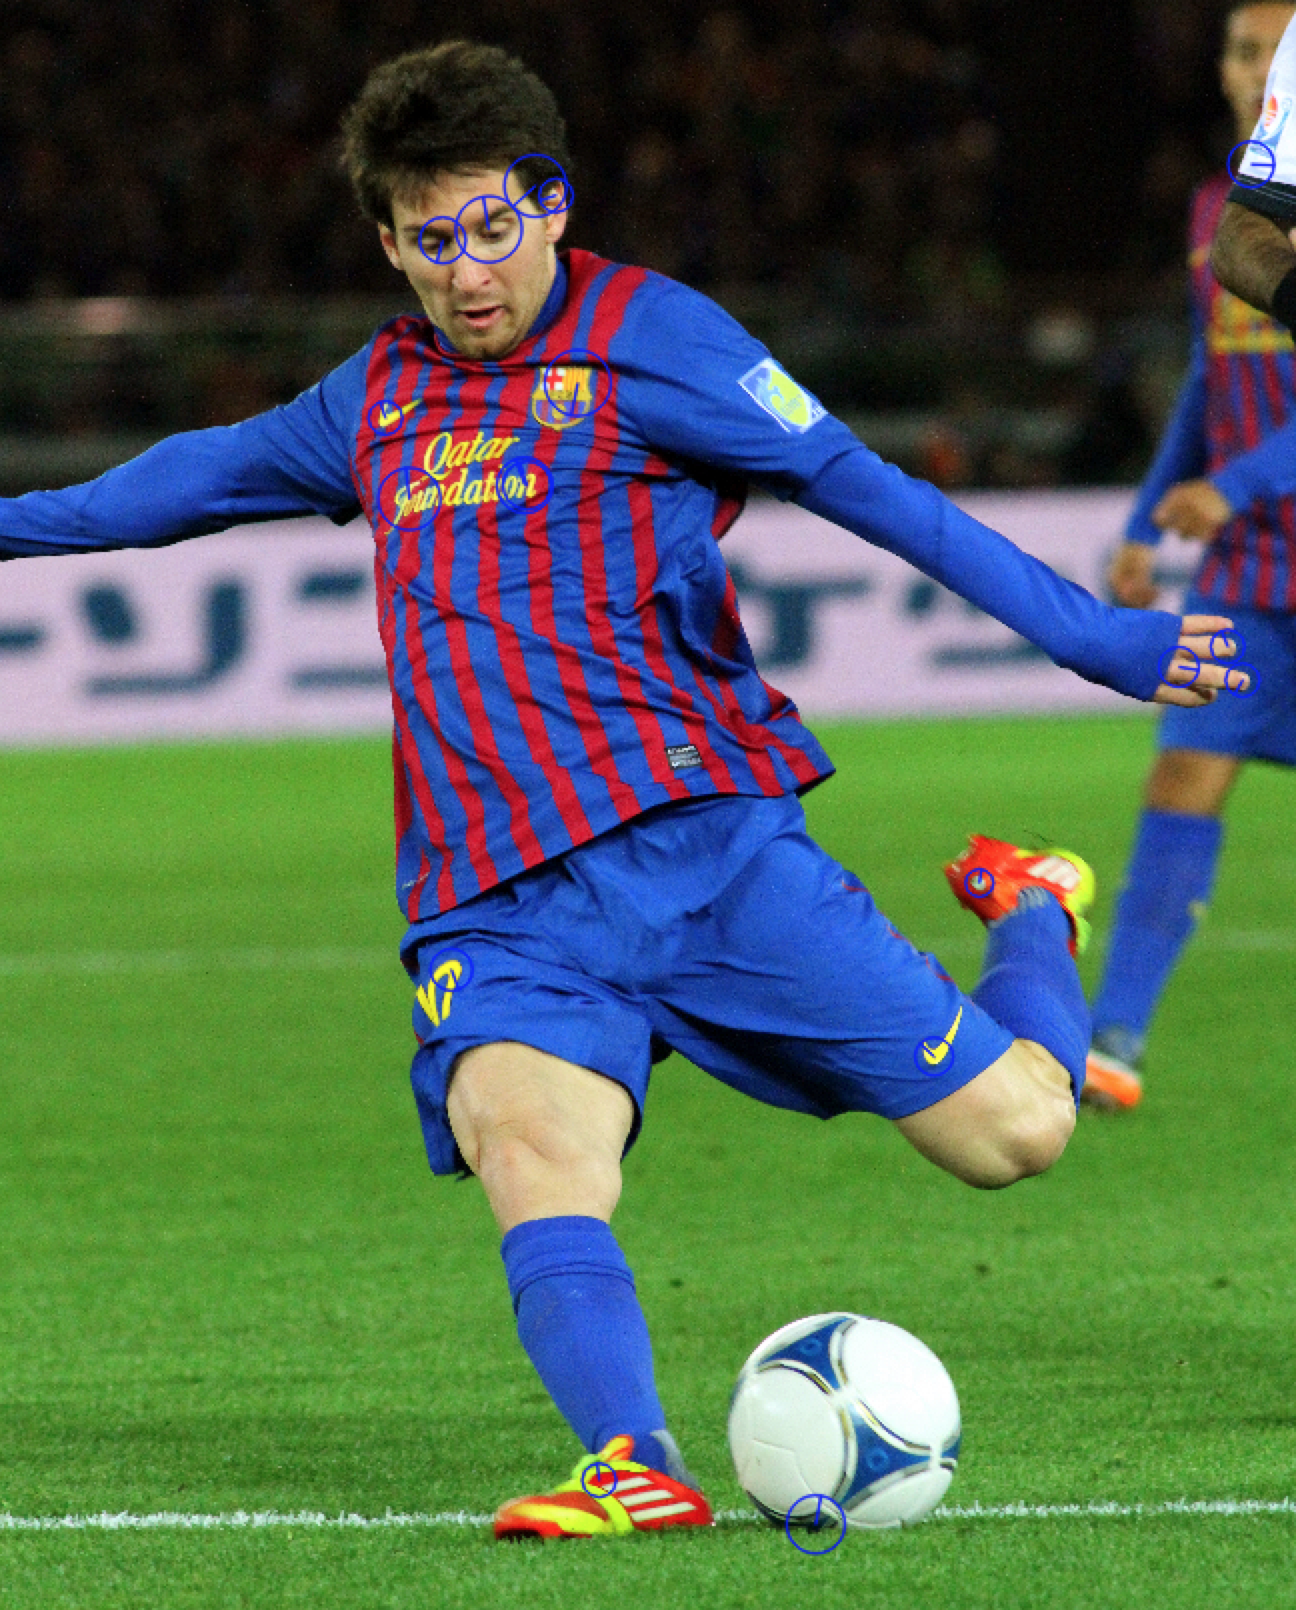
\includegraphics[width=.8\linewidth]{images/messiCornerSurf.png}
	\caption{SURF keypoints with\\ corner mask}
	\label{fig:messiCornerSurf}
\end{minipage}
\end{figure}


\section{Analysis of a pair of images}

In order to analyze a pair of images, we shall use the SIFT descriptors determined in the previous section.
The two sets of descriptors are compared in order to obtain the best matches between pairs of keypoints.
A distance is computed between each pair of keypoint descriptors, which is the Euclidian norm between the SIFT descriptors of the keypoints.
Experimentally, we have concluded that a match between two keypoints has a high similarity if the Euclidian norm is less than $100$.\\
For a pair of images, we first find the set of corner-mask keypoints and then compute the best matches between these keypoints. We shall keep only the best $10$ matches, and compute the arithmetic mean between the distances of these matches. As stated before, if this mean is smaller than $100$, the two images are considered similar. We shall name this algorithm the $pair\ similarity\ algorithm$.\\
Figure~\ref{fig:compareImages} shows the corresponding matches between two images with two different watermarks, one of which is rotated $90^o$ clockwise.

\begin{figure}[ht!]
\centering
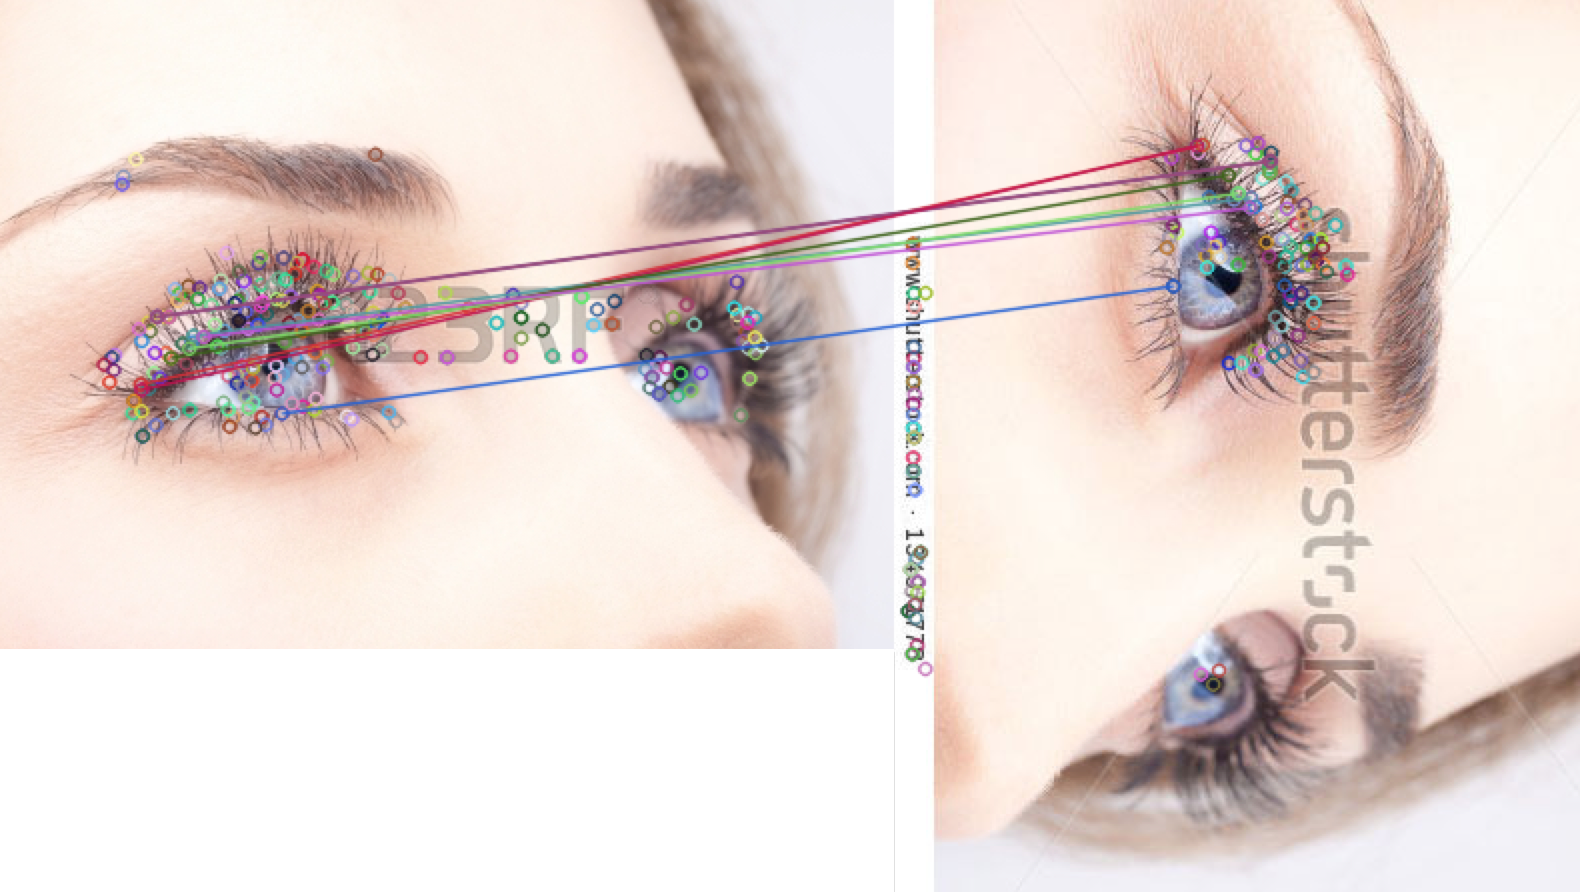
\includegraphics[width=.8\linewidth]{images/compare.png}
\caption{Comparison between two images}
\label{fig:compareImages}
\end{figure}
 
 
\section{Analysis of a set of images}

Suppose that we have a set of images, and we want to compare a test image with the set and detect whether we have a similar image within the set. Of course, the first possibility is the brut force one: we iterate through all the images and apply the $pair\ similarity\ algorithm$ described in the previous section.
Although this provides a correct result, it has a complexity of $O(number\_of\_images * image\_match\_time)$. We shall name this basic algorithm as the $linear\ algorithm$. Although this algorithm is very straightforward, its complexity is undesirable if the number of images becomes large (i.e more than $500$).
Moreover, most of the images in our set will likely have a big similarity distance with our searched image, so maybe we don't want to apply the full $pair\ similarity\ algorithm$.\\
Thus, we need to determine an efficient algorithm which can filter the initial set of images to a smaller set which contains the best possible candidates in terms of visual similarity.\\
The filtering algorithm is implemented as follows: we will maintain a maximum number of $M$ descriptors for each image in the initial set and create $P$ KD-trees with the set of descriptors of the initial images.
When a query for a test image arrives, we will compute its descriptors and then perform a $K$ nearest-neighbor search on each of our KD-trees. Then we will select the top $T$ images returned from the nearest neighbor searches and perform the $linear\ algorithm$. We shall name this algorithm the $kdtree\ algorithm$.\\
Of course, the important factors in the $kdtree\ algorithm$ are:
\begin{itemize}
	\item the values of the numbers $M$, $T$ and $K$ from the above description
	\item the metric used in selecting the top $T$ images from the nearest-neighbor search
	\item the metric used in selecting the $M$ descriptors from the input images to form the KD-tree
	\item $N$, the number of images that form a KD-tree
	\item $P$, the number of KD-trees, which can be determined from the total number of images and $N$.
\end{itemize}

We propose three metrics in for selecting the filtered images from the KD-tree based on the nearest-neighbor search:
\begin{itemize}
	\item the images with the largest number of descriptors returned from the search
	\item the images with the smallest average of the distance of the found descriptors
	\item the images with the largest distance between its descriptors and the average of all found descriptors (from all the images)
\end{itemize}
 
For the initial attempts, we have set the values of $M$, $T$ and $K$ to $40$, $10$ and $5$ and used the largest number of found descriptors as metric for selecting the filtered images from the KD-tree.\\
